\section{Auswertung}
\label{sec:Auswertung}
Die Auswertung wird mithilfe von Python erstellt. Dabei werden die Bibliotheken SciPy \cite{??}, NumPy \cite{??} und 
Uncertainties \cite{??} verwendet. 
\subsection{Überprüfung der Stabilitätbedingung und Untersuchung des Multimodenbetriebs}
Um die Stabilitätbedingung zu überprüfen wird zunächst eine Spiegelkonstellation mit einem flachen 
und einem konkaven $(r=\SI{1400}{\milli\meter})$ Spiegel verwendet. Laut Gleichung \eqref{eq:??}[g1*g2] ist die 
Stabilitätsbeding erfüllt, wenn der Abstand die Bedingung $d>\SI{1400}{\milli\meter})$ erfüllt.
Für diese Spiegelkonstellation konnte, bis zu einem Abstand von $d=\SI{980}{\milli\meter}$, ein Laserstrahl erzeugt werden.
Dies ist unter dem theoretischem Wert und wird in der Diskussion drauf eingegangen.\\
Die folgende Spiegelkonstellation besteht aus zwei konkaven Spiegeln mit jeweils einem Radius von $r=\SI{1400}{\milli\meter}$.
Die Stabilitätbedingung ist erfüllt, wenn der Abstand kleiner ist als $d = \SI{2800}{\milli\meter}$. 
Die Stabilitätbedingung kann bis zu einem Abstand von $\SI{1763}{\milli\meter}$ gezeigt werden. Für größere 
Abstände reicht der Versuchsaufbau nicht aus.
\subsubsection{Untersuchung des Multimodenbetriebs}
Um den Multimodenbetrieb zu untersuchen muss die Intensität mit einer schnellen Photodiode aufgenommen werden. Die 
Frequenzen der Intensitätsmaxima werden, in Abhängigkeit des Spiegelabstandes, mithilfe einer Fouriertransformation ermittelt. 
Die Messdaten sind in Tabelle \ref{tab:Multimodenbetrieb} aufgelistet.
\FloatBarrier
\begin{table}
  \centering
  \caption{Messdaten für die Untersuchung des Multimodenbetriebs.}
  \begin{tabular}{c c c c c}
    \toprule
    &$d=\SI{730}{\milli\meter}$&$d=\SI{848}{\milli\meter}$&$d=\SI{1350}{\milli\meter}$&$d=\SI{1763}{\milli\meter}$\\
    n&$f\,/\,\SI{}{\mega\hertz}$&$f\,/\,\SI{}{\mega\hertz}$&$f\,/\,\SI{}{\mega\hertz}$&$f\,/\,\SI{}{\mega\hertz}$\\
    \midrule
    1&$\num{236.6}$&$\num{176.6}$&$\num{119.0}$&$\num{88.0}$\\
    2&$\num{473.1}$&$\num{352.8}$&$\num{239.0}$&$\num{182.0}$\\
    3&$\num{709.8}$&$\num{527.5}$&$\num{357.0}$&$\num{272.0}$\\
    4&-&$\num{704.9}$&$\num{476.0}$&$\num{360.0}$\\
    5&-&$\num{879.1}$&$\num{596.0}$&$\num{452.0}$\\
    6&-&-&-&$\num{537.0}$\\
    7&-&-&-&$\num{627.0}$\\
  \end{tabular}
\end{table}
\FloatBarrier
Alle Intensitätsmaxima müssen die Gleichung $f = \frac{nc}{2d}$ erfüllen. Um das zu überprüfen kann die 
Frequenz gegen $n$ aufgetragen werden und eine lineare Ausgleichsgrade bestimmt werden. Die Steigung der 
Graden muss den Wert $\frac{c}{2d}$ haben.
Die Messdaten, Ausgleichsgraden und Theoriegraden sind in Abbildung \ref{fig:Multimodenbetrieb} abgebildet.
\FloatBarrier
\begin{figure}
  \centering
  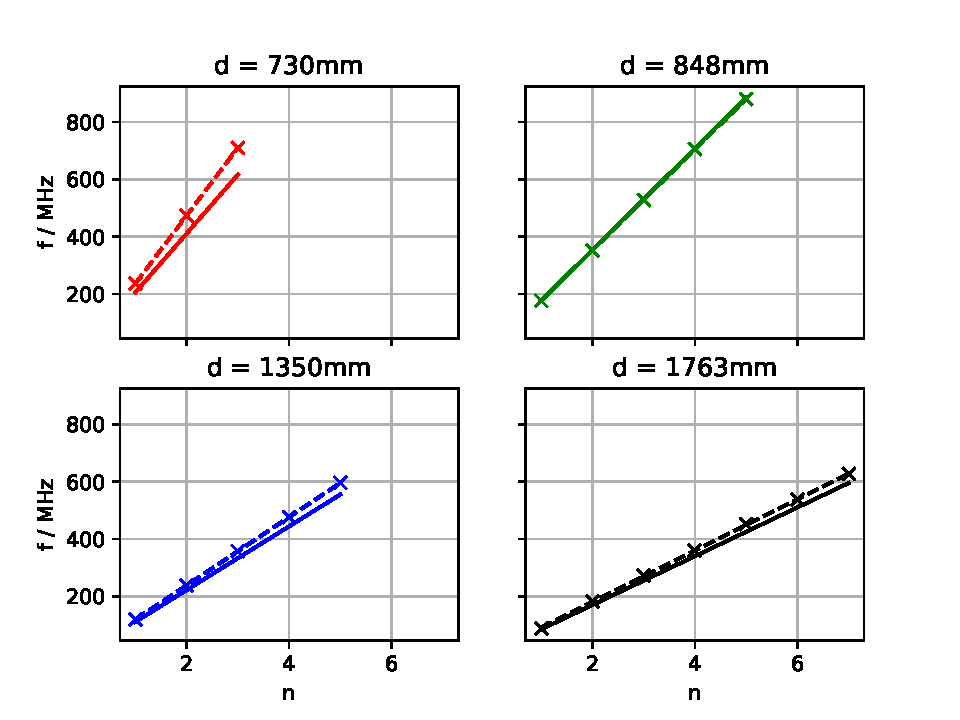
\includegraphics[width = \textwidth, keepaspectratio]{figure/Multimode.pdf}
  \caption{Plots der verschiedenen Abstände um die Bedingung der Frequenzen zu überprüfen. Hierbei sind die Kreuze die Messdaten, die gestrichene Linie die Ausgleichsgrade und die durchgezogene Linie die Theoriegrade.}
\end{figure}
\FloatBarrier
Die Steigungen der Ausgleichsgraden und die dazugehörigen theoretischen Werte sind in der Tabelle \ref{tab:Steigungen} aufgelistet.
\FloatBarrier
\begin{table}
  \centering
  \caption{Steigungen der Ausgleichsgraden und theoretische Werte zur Überprüfung des Multimodenbetriebs.}
  \label{tab:Steigungen}
  \begin{tabular}{c c c}
    \toprule
    Abstand $d\,/\,\SI{}{\milli\meter}$&Steigung $a_{\text{gemessen}}\,/\,\SI{}{\mega\hertz}$&Steigung $a_{\text{theoretisch}}\,/\,\SI{}{\mega\hertz}$\\
    \midrule
    $\num{730}$&$\num{236.60(6)}$&$\num{205.34}$\\
    $\num{843}$&$\num{175.71(25)}$&$\num{176.76}$\\
    $\num{1350}$&$\num{119.10(19)}$&$\num{111.03}$\\
    $\num{1763}$&$\num{89.5(4)}$&$\num{85.02}$\\
    \bottomrule
  \end{tabular}
\end{table}
\FloatBarrier
Keine der theoretischen Steigungen liegt in der Unsicherheit der gemessenen Steigung, allerdings sind die Größenordnungen 
in jedem der Fälle richtig.
\subsection{Beobachtung der TEM-Moden}
Um die TEM-Moden zu beobachten wird der Laserstrahl mit einer Streulinse vergrößert und mit einer Photodiode wird die 
Intensität senkrecht zur Strahlachse gemessen.
Es werden zwei Moden untersucht. 
\subsubsection{Beobachtung der \texorpdfstring{$\text{TEM}_{00}$}{T1}-Mode}
Die aufgenommenen Intensitäten sind in Tabelle \ref{tab:TEM00} aufgelistet.
\begin{table}
  \centering
  \caption{Aufgenommene Intensitäten für die Untersuchung der $\text{TEM}_{00}$-Mode.}
  \label{tab:TEM00}
  \begin{tabular}{c c}
    \toprule
    Abstand zum Strahlmittelpunkt $a\,/\,\SI{}{\milli\meter}$&Intensität $I \,/\,\SI{}{\micro\ampere}$\\
    \midrule
    $\num{-8.0}$&$\num{0.048}$\\
    $\num{-6.0}$&$\num{0.189}$\\
    $\num{-4.0}$&$\num{0.423}$\\
    $\num{-3.0}$&$\num{0.657}$\\
    $\num{-2.0}$&$\num{0.917}$\\
    $\num{0.0}$&$\num{1.316}$\\
    $\num{2.0}$&$\num{1.042}$\\
    $\num{4.0}$&$\num{0.545}$\\
    $\num{6.0}$&$\num{0.385}$\\
    $\num{8.0}$&$\num{0.35}$\\
    $\num{10.0}$&$\num{0.203}$\\
    $\num{12.0}$&$\num{0.39}$\\
    \bottomrule
  \end{tabular}
\end{table}
\FloatBarrier
Wie in Abbildung \ref{fig:TEM00} zu sehen ist, wird an die gemessene Daten eine Gaußfunktion
\begin{equation}
  \label{eq:Gaußfunktion}
  G(x)= G_{0}\exp{\left(-\left(\frac{x-\mu}{\sqrt{2}\sigma}\right)^2\right)}
\end{equation} 
gefittet. 
\FloatBarrier
\begin{figure}
  \centering
  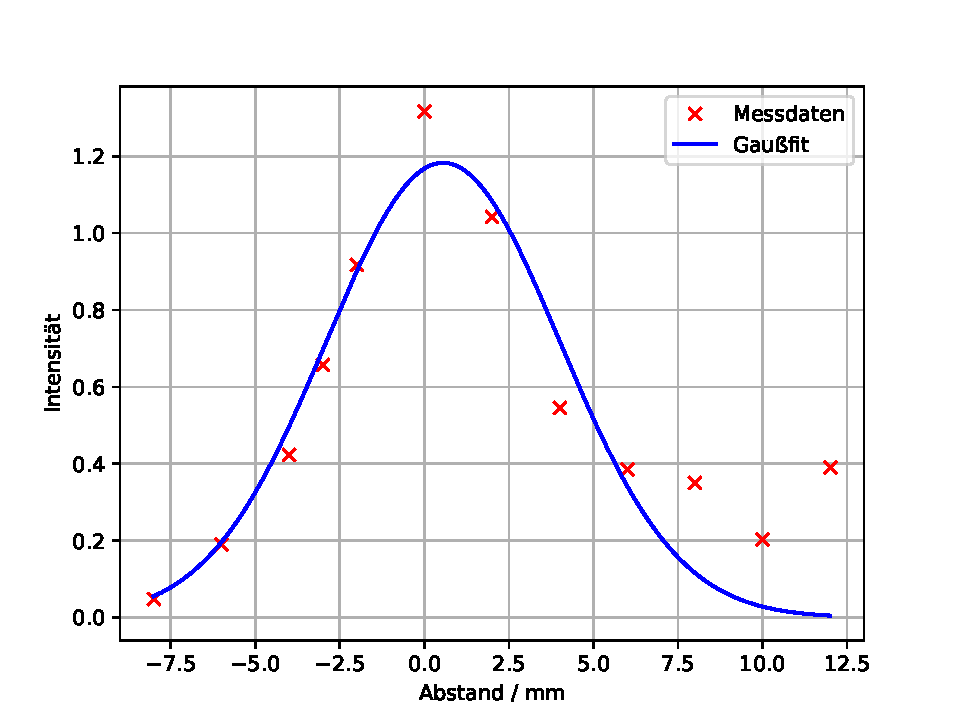
\includegraphics[width = \textwidth, keepaspectratio]{figure/TEM00.pdf}
  \caption{Gemessene Daten und Fitfunktion der $\text{TEM}_{00}$-Mode.}
  \label{fig:TEM00}
\end{figure}
\FloatBarrier
Die Fitparameter der Funktion sind
\begin{align*}
  G_{0}=&\SI{3.5(4)}{\micro\ampere}\\
  \mu =& \SI{1.18(13)}{\milli\meter}\\
  \sigma =& \SI{0.6(4)}{\milli\meter}.
\end{align*}
\subsubsection{Beobachtung der \texorpdfstring{$\text{TEM}_{10}$}{T1}-Mode}
Um die $\text{TEM}_{10}$-Mode zu sehen muss ein dünner Draht in die Mitte des Strahles eingesetzt werden. Die 
so aufgenommenen Daten sind in Tabelle \ref{tab:TEM01} aufgelistet.
\begin{table}
  \centering
  \caption{Aufgenommene Intensitäten für die Untersuchung der $\text{TEM}_{10}$-Mode.}
  \label{tab:TEM01}
  \begin{tabular}{c c}
    \toprule
    Abstand zum Strahlmittelpunkt $a\,/\,\SI{}{\milli\meter}$&Intensität $I \,/\,\SI{}{\micro\ampere}$\\
    \midrule
    $\num{12.0}$&$\num{0.305}$\\
    $\num{10.0}$&$\num{0.428}$\\
    $\num{8.0}$&$\num{0.545}$\\
    $\num{6.0}$&$\num{0.462}$\\
    $\num{4.0}$&$\num{0.293}$\\
    $\num{2.0}$&$\num{0.144}$\\
    $\num{0.0}$&$\num{0.002}$\\
    $\num{-2.0}$&$\num{0.046}$\\
    $\num{-3.0}$&$\num{0.081}$\\
    $\num{-4.0}$&$\num{0.105}$\\
    $\num{-6.0}$&$\num{0.2}$\\
    $\num{-8.0}$&$\num{0.215}$\\
    $\num{-10.0}$&$\num{0.152}$\\
    $\num{-12.0}$&$\num{0.076}$\\
    $\num{-14.0}$&$\num{0.014}$\\
    \bottomrule
  \end{tabular}
\end{table}
\FloatBarrier
In den Daten sind zwei Maxima zu erkennen, daher wird pro Maxima eine Gaußfunktion angepasst. Diese beiden Gaußfunktionen werden
addiert um die gesamt Verlauf darzustellen.
\FloatBarrier
\begin{figure}
  \centering
  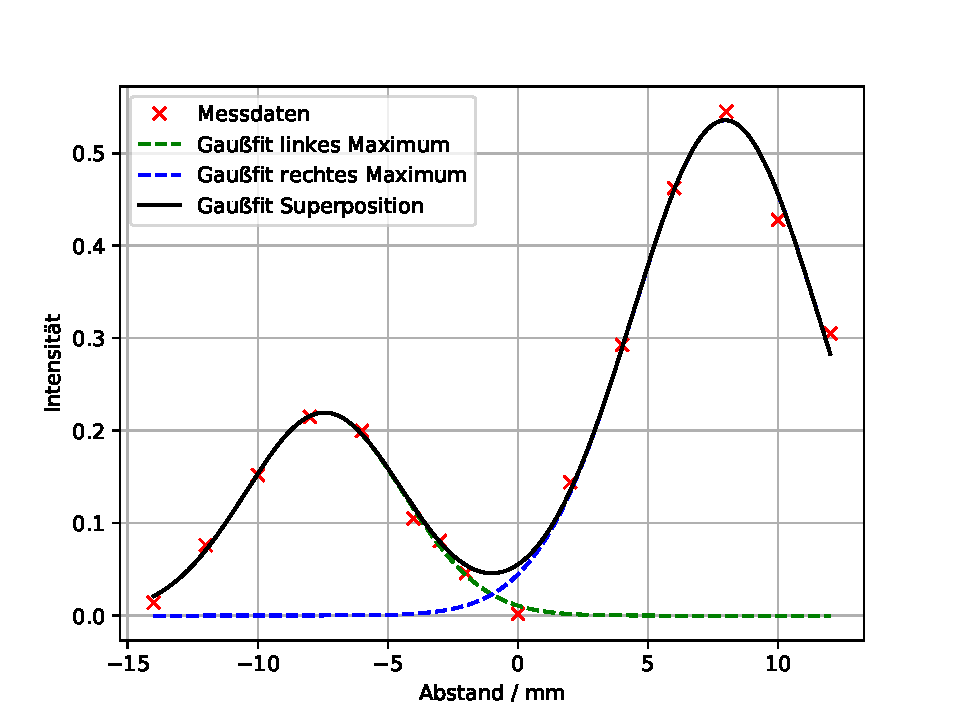
\includegraphics[width = \textwidth, keepaspectratio]{figure/TEM01.pdf}
  \caption{Gemessene Daten und Fitfunktion der $\text{TEM}_{10}$-Mode.}
\end{figure}
\FloatBarrier
Die Fitparameter der beiden Funktionen sind 
\begin{align*}
G_{0 \text{links}}=&\SI{0.220(5)}{\micro\ampere}\quad &G_{0 \text{rechts}}=&\SI{0.536(20)}{\micro\ampere}\\
\mu_{\text{links}} =& \SI{-7.45(8)}{\milli\meter}\quad &\mu_{\text{rechts}} =& \SI{7.97(17)}{\milli\meter}\\
\sigma_{\text{links}} =& \SI{3.03(8)}{\milli\meter}\quad &\sigma_{\text{rechts}} =& \SI{3.57(19)}{\milli\meter}.
\end{align*}
\subsection{Bestimmung der Polarisation}
Um die Polarisation zu messen wird zwischen dem Auskoppelspiegel und dem Intensitätsmessgerät eine Polarisationsfilter 
aufgestellt. Die gemessenen Intensitäten sind in Tabelle \ref{tab:Polarisation} aufgelistet.
\FloatBarrier
\begin{table}
  \centering
  \caption{Intensität in Abhängigkeit des Winkels des Polarisationsfilters.}
  \label{tab:Polarisation}
  \begin{tabular}{c c}
    \toprule
    Winkel $\varphi \,/\,\SI{}{\radian}$&Intensität $I\,/\,\SI{}{\milli\watt}$\\
    \midrule
    $\num{0.0}$&$\num{0.0204}$\\
    $\num{0.17}$&$\num{0.1355}$\\
    $\num{0.35}$&$\num{0.388}$\\
    $\num{0.52}$&$\num{0.756}$\\
    $\num{0.7}$&$\num{1.120}$\\
    $\num{0.87}$&$\num{1.564}$\\
    $\num{1.05}$&$\num{1.879}$\\
    $\num{1.22}$&$\num{2.193}$\\
    $\num{1.4}$&$\num{2.324}$\\
    $\num{1.57}$&$\num{2.345}$\\
    $\num{1.75}$&$\num{2.204}$\\
    $\num{1.92}$&$\num{1.984}$\\
    $\num{2.09}$&$\num{1.614}$\\
    $\num{2.27}$&$\num{1.250}$\\
    $\num{2.44}$&$\num{0.814}$\\
    $\num{2.62}$&$\num{0.464}$\\
    $\num{2.79}$&$\num{0.186}$\\
    $\num{2.97}$&$\num{0.023}$\\
    $\num{3.14}$&$\num{0.010}$\\
    \bottomrule
  \end{tabular}
\end{table} 
\FloatBarrier
Durch die gemessenen Daten kann die Funktion
\begin{equation}
  \label{eq:Sin2}
  I(\varphi)=A\cdot\sin{\left(B\left(\varphi+C\right)\right)}^2 + D
\end{equation}
gefittet werden.
Die Messdaten und die Fitfunktion ist in Abbildung \ref{fig:Polarisation} dargestellt.
\FloatBarrier
\begin{figure}
  \centering
  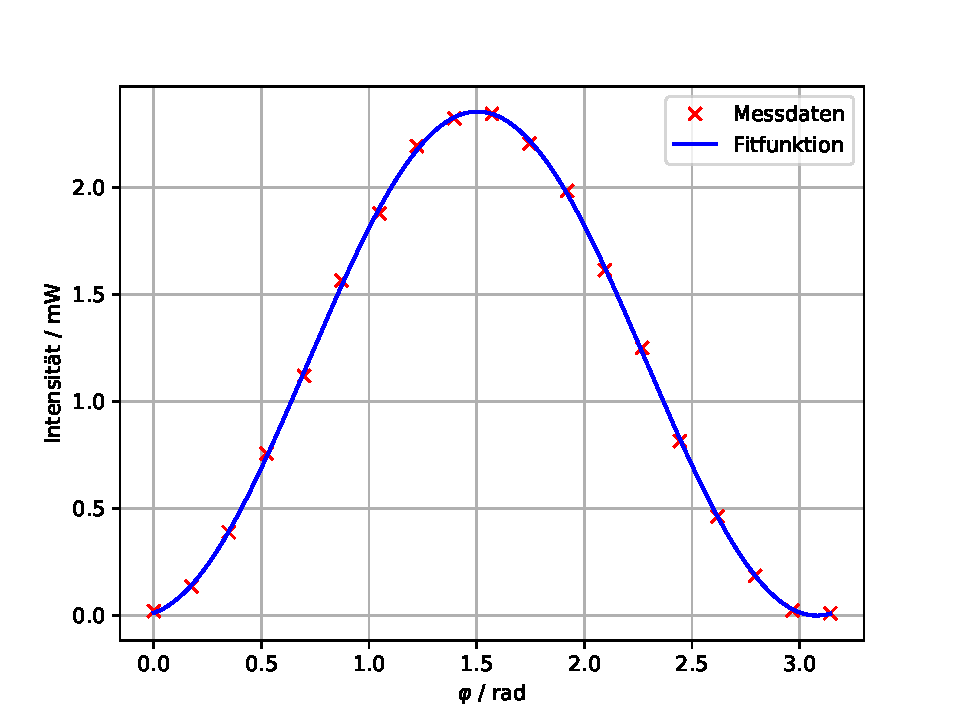
\includegraphics[width= \textwidth, keepaspectratio]{figure/Polarisation.pdf}
  \caption{Messdaten und Fitfunktion für die Bestimmung der Polaristation.}
  \label{fig:Polarisation}
\end{figure}
\FloatBarrier
Wie in Abbildung \ref{fig:Polarisation} zu sehen ist, lassen sich die Messdaten gut mit einer Funktion der Form \eqref{eq:Sin2}
beschreiben.
Die Fitparameter sind 
\begin{align*}
  A=&\SI{2.355(10)}{\milli\watt} &B=&\num{0.996(5)}\\
  C=&\SI{0.074(7)}{\radian} &D=&\SI{-0.001(9)}{\milli\watt}.
\end{align*}
\subsection{Bestimmung der Wellenlänge}
Für die Bestimmung der Wellenlänge werden nacheinander zwei verschiedene Gitter in den Strahl gesetzt und die damit entstandenen 
Beugungsmaxima vermessen.
Auf den Gittern ist die Anzahl an Linien pro Millimeter angegeben. Um den Gitterabstand zu bestimmen wird der Wert mit dem 
Faktor $\num{1000}$ multipliziert, dadurch wird die Anzahl an Linien pro Meter bestimmt und der Gitterabstand in Metern ist 
das Inverse des Wertes.
Die Gitterabstände der beiden Gitter sind in der Tabelle \ref{tab:Gitterabstand} aufgelistet.
\FloatBarrier
\begin{table}
  \centering
  \caption{Daten der verwendeten Gitter.}
  \label{tab:Gitterabstand}
  \begin{tabular}{c c c}
    \toprule
    Gitter&\#Linien / $\SI{}{1\per\milli\meter}$&Gitterabstand $a\,/\,\SI{}{\meter}$\\
    \midrule
    A&$\num{100}$&$\num{1e-5}$\\
    B&$\num{600}$&$\num{1.67e-6}$\\
    \bottomrule
  \end{tabular}
\end{table}
\FloatBarrier
Die gemessenen Positionen der Beugungsmaxima sind in der Tabelle \ref{tab:Maxposi} aufgelistet. Bei der Messung der 
Beugungsmaxima von Gitter A war der Abstand von Schirm und Gitter $d=\SI{25}{\centi\meter}$ und bei Gitter B $d=\SI{5}{\centi\meter}$.
Mit dem Gitterabstand $a$, der Position der Beugungsmaxima $b_{\text{n}}$ relativ zum Strahlmittelpunkt und dem Abstand $d$ kann mit den
Gleichung 
\begin{equation*}
  \varphi_{\text{n}}=\arctan{\left(\frac{b_{\text{n}}}{d}\right)},\qquad \lambda = a\cdot\frac{\sin{\left(\varphi_{\text{n}}\right)}}{\text{n}}
\end{equation*}
die Wellenlänge $\lambda$ bestimmt werden. Die Winkel $\varphi_{\text{n}}$ und die Wellenlänge sind ebenfalls in Tabelle \ref{tab:Maxposi} aufgelistet.
\FloatBarrier
\begin{table}
  \centering
  \caption{Messdaten für die Bestimmung der Wellenlänge des Lasers. Die Positionen der Maxima sind relativ zur Strahlachse, daher werden nur die Absolutwerte angegeben.}
  \label{tab:Maxposi}
  \begin{tabular}{c c c c| c c c}
    \toprule
    &\multicolumn{3}{c}{Gitter A}&\multicolumn{3}{c}{Gitter B}\\
    \cmidrule(lr){2-4} \cmidrule(lr){5-7}
    Position n&$b_{\text{n}}\,/\,\SI{}{\centi\meter}$&$\varphi_{\text{n}}\,/\,\SI{}{radian}$&$\lambda\,/\,\SI{}{\nano\meter}$&$b_{\text{n}}\,/\,\SI{}{\centi\meter}$&$\varphi_{\text{n}}\,/\,\SI{}{radian}$&$\lambda\,/\,\SI{}{\nano\meter}$\\
    \midrule
    1&$\num{1.6}$&$\num{0.064}$&$\num{638.7}$&$\num{2.2}$&$\num{0.415}$&$\num{671.2}$\\
    1&$\num{1.6}$&$\num{0.064}$&$\num{638.7}$&$\num{2.2}$&$\num{0.415}$&$\num{671.2}$\\
    2&$\num{3.2}$&$\num{0.127}$&$\num{634.8}$&$\num{6.0}$&$\num{0.876}$&$\num{640.2}$\\
    2&$\num{3.2}$&$\num{0.127}$&$\num{634.8}$&$\num{6.9}$&$\num{0.944}$&$\num{674.8}$\\
    3&$\num{4.9}$&$\num{0.194}$&$\num{641.1}$&-&-&-\\
    3&$\num{4.9}$&$\num{0.194}$&$\num{641.1}$&-&-&-\\
    4&$\num{6.6}$&$\num{0.258}$&$\num{638.1}$&-&-&-\\
    4&$\num{6.7}$&$\num{0.262}$&$\num{647.2}$&-&-&-\\
    \bottomrule
  \end{tabular}
\end{table}
\FloatBarrier 
Die Wellenlänge aus \ref{tab:Maxposi} können noch gemittelt werden, dadurch werden die Wellenlängen $\lambda_{\text{A}}=\SI{639(4)}{\nano\meter}$ und
$\lambda_{\text{B}}=\SI{664(14)}{\nano\meter}$ berechnet. Der Mittelwert dieser beiden Wellenlängen beträgt $\lambda=\SI{652(7)}{\nano\meter}$.